\documentclass[a4paper, 12pt, twoside]{article}

%%%%%%%%%%%%%%%%%%%%%%%%% PACOTES %%%%%%%%%%%%%%%%%%%%%%%%%%%%%%%%%%

\usepackage[inner = 3cm, outer = 2cm, top = 3cm, bottom= 2cm]{geometry}
\usepackage[utf8]{inputenc}
\usepackage[T1]{fontenc}
\usepackage[brazil]{babel}
\usepackage{hyphenat}
\usepackage{lmodern}
\usepackage{graphicx}
\usepackage{url} % Pacote para formatar URLs
\usepackage{nomencl} 
\usepackage{color}
\usepackage{enumitem}
\usepackage{microtype}
\usepackage{lipsum}	
\usepackage{amsfonts,amsmath,amssymb}
\usepackage{booktabs}
\nocite{*}
\bibliographystyle{plain}
\bibliography{referencias}


% Configuração dos parágrafos
\usepackage{indentfirst}
\setlength{\parindent}{1.25cm}

% Configuração do espaçamento
\usepackage{setspace}

% Configuração de alinhamento de texto
\usepackage{ragged2e}

% Configuração de numeração de página
\usepackage{fancyhdr}
\fancyhf{}
\rhead{\thepage}
\cfoot{}
\renewcommand{\headrulewidth}{0pt} % zera linha de cabeçalho
\pagestyle{fancy}
\setlength{\headheight}{15pt}

% Configuração da Fonte
\usepackage{times} % Fonte: Times New Roman 

\usepackage[xcolor]{xcolor}

% Formatando Sections
\usepackage{mfirstuc}

\usepackage{titlesec}
\titleformat{\section}{\normalfont\fontsize{12}{12}\bfseries\MakeUppercase}{\thesection}{0.5em}{}

\titleformat{\subsection}{\normalfont\fontsize{12}{12}\bfseries}{\thesubsection}{0.5em}{\capitalisewords}

\titleformat{\subsubsection}{\normalfont\fontsize{12}{12}\bfseries\itshape}{\thesubsubsection}{0.5em}{\capitalisewords}

%PACOTE DE CITAÇÕES
\usepackage[style=abnt,backend=biber]{biblatex} % Usa biblatex para citações e referências
\addbibresource{referencias.bib} % Nome do arquivo .bib
\usepackage{changepage}
\usepackage{ifoddpage}

% Define ambiente quote para citações diretas com mais de 3 linhas
\newenvironment{myquote}{\par\fontsize{10pt}{12pt}\selectfont\begin{adjustwidth}{4cm}{0pt}}{\end{adjustwidth}\par}

% PACOTES ESSENCIAIS
\usepackage{graphicx}
\usepackage{float}
\usepackage{caption}
\usepackage{xurl}
\usepackage{hyperref}

% Define o tamanho da fonte para as legendas
\DeclareCaptionFont{mycaptionfont}{\fontsize{10pt}{12pt}\selectfont}

% Aplica o tamanho da fonte definido às legendas de figuras
\captionsetup{font=mycaptionfont}

% Redefine o separador das legendas para travessão (-)
\DeclareCaptionLabelSeparator{myhyphen}{ --- }
\captionsetup{font=mycaptionfont, labelsep=myhyphen}

% Preencha as informações do título, subtítulo, autor e orientador aqui
\newcommand{\titulo}{Análise de casos de Dengue no Brasil: impactos, sintomas e a influência dos casos na Pandemia da COVID-19}

\newcommand{\orientador}{Rafael de Pinho André}
\newcommand{\autor}{Alex Júnio Maia de Oliveira}
\newcommand{\autordois}{Bruno Ferreira  Salvi}
\newcommand{\autortres}{João Pedro Jerônimo de Oliveira}
\newcommand{\autorquatro}{Matheus Vilarino de Sousa Pinto}
\newcommand{\autorcinco}{Thalis Ambrosim Falqueto}

\begin{document} %Início do Documento

\singlespacing % espaçamento simples
\justifying % texto justificado

%%%%%%%%%%%%%%%%%%%%%%%% CONFIG. DO TÍTULO %%%%%%%%%%%%%%%%%%%%%%%%

\vspace*{0.5cm} %Espaçamento Superior do Título
\begin{center} %Inicia a centralização
\textbf{\MakeUppercase{\titulo}}       
\end{center} %Finaliza a centralização

%%%%%%%%%%%%%%%%%%%%%%%%% AUTORES E ORIENTADOR %%%%%%%%%%%%%%%%%%%%%%%%%

\begin{flushright}
\orientador \\

\autor  \\
\autordois  \\
\autortres  \\
\autorquatro  \\
\autorcinco \\
 
\end{flushright}

%%%%%%%%%%%%%%%%%%%%% RESUMO E ABSTRACT %%%%%%%%%%%%%%%%%%%%%%%%%%%%%%

\begin{center}
\vspace*{0.5cm}
\textbf{\MakeUppercase{Resumo}}
\end{center}


\noindent 
O presente artigo tem como objetivo geral analisar o conjunto de dados disponibilizado pelo SINAN (Sistema de Informação de Agravos de Notificação), coletado pelo Sistema Único de Saúde (SUS), referente aos casos de dengue registrados no Brasil entre 2021 e 2024. Foram elaboradas cinco hipóteses principais para investigar possíveis correlações entre as variáveis do dataset, com o objetivo de gerar insights que contribuam para uma compreensão mais profunda dos casos de dengue no período analisado. A metodologia envolve etapas como o pré-processamento dos dados, a análise exploratória e a validação ou refutação de hipóteses, utilizando técnicas de estatística descritiva e visualização de dados. O estudo também busca identificar padrões e observações relevantes, empregando ferramentas nativas do \emph{Python}, como \emph{pandas} e \emph{numpy}, além de bibliotecas de visualização como \emph{matplotlib}, \emph{seaborn} e \emph{streamlit}.  

\noindent \textbf{Palavras-chave:} Dengue; Python; análise de dados.

\section{Introdução}

Atualmente, há diversos conjuntos de dados relacionados à saúde disponíveis na Internet, abordando uma ampla gama de informações, como doenças, tratamentos, vacinas, hospitais, entre outros. O conjunto de dados "\textit{DADOS SUS SINAN DENGUE (2021-2024)}" oferece uma base concisa com informações sobre os casos de dengue registrados no Sistema Único de Saúde (SUS) entre 2021 e 2024 no Brasil. Esse dataset se configura como uma valiosa fonte para investigar as correlações entre diferentes variáveis, como tipos de doenças, datas de entrada e saída, e características dos pacientes.

Compreender as relações entre essas variáveis pode gerar insights importantes para hospitais, clínicas e até mesmo para os próprios pacientes, auxiliando na tomada de decisões estratégicas e na identificação de padrões relacionados à doença em questão. Por exemplo, seria possível identificar se existe algum sintoma principal que se correlaciona com o agravamento da doença ou óbito? Alguns sintomas podem estar associados à faixa etária dos pacientes? E, ainda, qual seria a influência da pandemia de Covid-19 no aumento ou diminuição dos casos de dengue?

O objetivo deste estudo é realizar uma análise de associação, e não de causalidade, entre os fatores presentes no conjunto de dados mencionado. O artigo segue a seguinte estrutura: na seção 2, é apresentada a metodologia utilizada, com uma descrição detalhada do dataset e das técnicas de manipulação de dados aplicadas. Na seção 3, são discutidos os resultados obtidos com a análise das relações entre as variáveis, seguidos por uma reflexão sobre os achados e possíveis direções para estudos mais aprofundados. Por fim, a seção 4 encerra o artigo com uma conclusão que destaca as limitações do estudo e propõe sugestões para futuras pesquisas.

\section{Desenvolvimento}
A base de dados disponibilizada gratuitamente no "\textit{DADOS SUS SINAN DENGUE (2021-2024)}" \cite{henrique2023} contém uma ampla gama de informações sobre os casos de dengue registrados em todo o Brasil. As principais variáveis incluem características dos pacientes, datas das ocorrências e uma variedade de sintomas associados à doença. As análises foram conduzidas na linguagem de programação \emph{Python}, utilizando bibliotecas externas como Numpy, Pandas, Seaborn, Matplotlib e Geopandas, além de bibliotecas \emph{built-in} como os e sys.

Para a análise exploratória dos dados, foram aplicados conceitos de estatística descritiva\footnote{BUSSAB, Wilton de Oliveira; MORETTIN, Pedro Alberto. Estatística básica. 9. ed. São Paulo: Saraiva, 2017}, como coeficiente de contingência, correlação e covariância, para explorar as relações entre as variáveis. Esses procedimentos possibilitaram uma compreensão mais aprofundada das interações entre os diferentes fatores e ajudaram na validação ou refutação das hipóteses formuladas.

O estudo tem como objetivos analisar os casos de dengue e compreender sua distribuição geral no cenário brasileiro, averiguar a sua correlação com o período pandêmico e fomentar a pesquisa no âmbito da prevenção da doença, ambrangendo tecnologias, análises de dados e identificação de padrões para a melhora do bem-estar da população brasileira e, por conseguinte, as populações afetadas pela enfermidade.

Espera-se que este estudo contribua de forma significativa para o avanço do conhecimento científico sobre a dengue, fornecendo abordagens relevantes para a formulação de políticas públicas mais eficazes e para o aprimoramento das estratégias de controle e prevenção da doença.
\\
\section{RESULTADOS E DISCUSSÕES}

Como parte principal do artigo, o desenvolvimento enfatizará a legitimação das teorias propostas na introdução, buscando um entendimento completo da base de dados escolhida.


%%%%%%%%% Hipótese 1 %%%%%%%%%
\subsection{Hipótese 1}
\emph{"Quais são os conjuntos de sintomas que mais levam à internação ou óbito do paciente?"}

Sabe-se que a dengue é uma doença caracterizada por uma ampla gama de sintomas e, dessa maneira, seria natural se questionar qual seria o conjunto de sintomas mais associado à piora do estado de saúde dos pacientes.
Foram levados em conta vários sintomas, sendo os principais deles :
\begin{itemize}
    - Febre Alta : reação de defesa do organismo, caracterizada pela elevação da temperatura corporal entre 39 a 40 graus celsius;\\
    - Mialgia : dores musculares intensas; \\
    - Dor de Cabeça : dor intensa na região frontal;\\
    - Hipertensão : niveis elevados de pressão arterial;\\ 
    - Naúsea : enjôo seguido de fraqueza e falta de apetite;\\
    - Vômito : quadros de vômitos persistentes e dores aabdominais;\\
    - Renal : prejudicação do sistema renal do indivíduo.\\
\end{itemize} 
Aqui está a tabela dos sintomas ordenada pela razão de óbito:

\begin{table}[H]
    \centering
    \caption{Dados de Sintomas e Razão de Óbito - Parte 1}
    \begin{tabular}{@{}lccc@{}}
        \toprule
        \textbf{Conjunto de Sintomas} & \textbf{Óbitos} & \textbf{Ocorrências} & \textbf{Razão \%} \\ 
        \midrule
        Renal & 61 & 668 & 9.13 \\
        Hematológico & 41 & 515 & 7.96 \\
        Hipertensão & 485 & 7669 & 6.32 \\
        Hepatopatia & 19 & 403 & 4.71 \\
        Vômito & 448 & 13493 & 3.32 \\
        Dor nas Costas & 232 & 6891 & 3.37 \\
        Petequias & 97 & 3224 & 3.01 \\
        Náusea & 462 & 16249 & 2.84 \\
        Leucopenia & 157 & 5563 & 2.82 \\
        Mialgia & 728 & 26346 & 2.76 \\
        Artralgia & 146 & 5356 & 2.73 \\
        Febre & 773 & 28933 & 2.67 \\
        Cefaleia & 539 & 22860 & 2.36 \\
        Dor Retro & 174 & 7696 & 2.26 \\
        Conjuntivite & 23 & 1009 & 2.28 \\
        Exantema & 89 & 4143 & 2.15 \\
        Artrite & 68 & 2026 & 3.36 \\ 
        \bottomrule
    \end{tabular}
    \label{tab:symptom_data_1}
\end{table}

\begin{table}[H]
    \centering
    \caption{Dados de Sintomas e Razão de Óbito - Parte 2}
    % Início do redimensionamento
    \resizebox{0.7\textwidth}{!}{ % Redimensiona para caber na largura do texto
        \begin{tabular}{@{}lccc@{}}
            \toprule
            \textbf{Conjunto de Sintomas} & \textbf{Óbitos} & \textbf{Ocorrências} & \textbf{Razão \%} \\ 
            \midrule
            Conjuntivite | Hematológico & 7 & 46 & 15.22 \\
            Dor nas Costas | Hematológico & 17 & 117 & 14.53 \\
            Artralgia | Hematológico & 16 & 108 & 14.81 \\
            Dor nas Costas | Renal & 19 & 169 & 11.24 \\
            Renal | Hipertensão & 45 & 417 & 10.79 \\
            Vômito | Renal & 28 & 273 & 10.26 \\
            Exantema | Renal & 7 & 70 & 10.00 \\
            Petequias | Renal & 6 & 61 & 9.84 \\
            Vômito | Hematológico & 20 & 209 & 9.57 \\
            Cefaleia | Hematológico & 31 & 329 & 9.42 \\
            Febre | Renal & 48 & 517 & 9.28 \\
            Artrite | Renal & 6 & 64 & 9.38 \\
            Mialgia | Renal & 44 & 483 & 9.11 \\
            Cefaleia | Renal & 33 & 363 & 9.09 \\
            Conjuntivite | Hepatopatia & 3 & 34 & 8.82 \\
            Dor Retro | Renal & 12 & 137 & 8.76 \\
            Febre | Hematológico & 39 & 447 & 8.72 \\
            Petequias | Hepatopatia & 5 & 62 & 8.06 \\
            Mialgia | Hematológico & 30 & 379 & 7.92 \\
            Náusea | Renal & 27 & 345 & 7.83 \\
            Hematológico | Hipertensão & 14 & 185 & 7.57 \\
            Náusea | Hematológico & 19 & 259 & 7.34 \\
            Artralgia | Renal & 8 & 110 & 7.27 \\
            \bottomrule
        \end{tabular}
    } % Fim do redimensionamento
    \label{tab:symptom_data_2}
\end{table}

Baseando-se nessa limitada base de dados, poderíamos supor a possível existência de alguns conjuntos de doenças que estariam correlacionados a internação ou óbito do paciente. Porém, se percebe que, para que uma análise correta fosse feita, seriam necessários dados que nos levassem a conhecer o período em que certo paciente apresentou um sintoma em específico. Aqui listamos alguns pontos importantes :

\begin{flushleft}
\begin{itemize}[nosep]
    \item \textbf{Fator de Comorbidade:} Pacientes que apresentaram sintomas mais graves ou letais podem ter tido condições de saúde preexistentes (como diabetes ou hipertensão) que aumentaram o risco de morte. Esses fatores não estariam explicitamente representados apenas nos sintomas de dengue.
    
    \item \textbf{Confusão entre Sintomas e Gravidade da Doença:} Alguns sintomas mais graves podem aparecer em pacientes já em estágio avançado da doença, mas isso não implica que esses sintomas causam a morte. Na verdade, eles são apenas indicadores de que a doença já está em uma fase mais séria.
    
    \item \textbf{Variabilidade dos Sintomas e Tratamento:} Em muitos casos, sintomas que parecem mais letais podem estar associados a um atraso no tratamento ou na detecção da dengue, e não ao sintoma em si.
    
    \item \textbf{Problema de Multicolinearidade:} Alguns sintomas podem estar altamente correlacionados entre si, de modo que sintomas similares ou relacionados acabam ocorrendo juntos. Isso pode dar uma falsa impressão de que conjuntos específicos de sintomas são letais, quando, na verdade, são sintomas de uma mesma condição subjacente.
    
    \item \textbf{Viés de Seleção:} A análise pode ter um viés se apenas pacientes com sintomas graves foram incluídos na base de dados, ou se o número de pacientes recuperados é desproporcional. Isso afeta a validade dos sintomas identificados como “mais letais”.
\end{itemize}
\end{flushleft} 

Para concluir essa análise, observa-se que uma investigação precisa sobre a letalidade dos sintomas de dengue requer dados mais completos e específicos, especialmente sobre a cronologia dos sintomas, histórico de comorbidades e contexto clínico de cada paciente. Em uma análise preliminar, apenas relacionar conjuntos de sintomas com a mortalidade pode levar a interpretações equivocadas, como evidenciado pelos pontos listados.

Assim, conclui-se que uma análise mais robusta dependeria de um conjunto de dados mais abrangente e de técnicas estatísticas que permitam isolar os efeitos específicos de cada sintoma, levando em conta fatores como o estado de saúde prévio, o estágio da doença e a qualidade e o tempo de acesso ao tratamento. Dessa forma, poderíamos realmente identificar quais sintomas têm maior relevância na gravidade e letalidade da dengue, auxiliando médicos a focarem nos sinais mais críticos em pacientes com esse diagnóstico.

%%%%%%%%% Hipótese 2 %%%%%%%%%

\subsection{Hipótese 2} 

\emph{Existe um padrão temporal na ocorrência dos casos de dengue?A Região Norte do Brasil apresentou o maior número de casos de dengue? Em qual localidade a taxa de mortalidade é mais elevada?}

Nessa hipótese, vamos analisar as colunas do dataset total (\textit{sinan\_dengue\_sample\_total.csv}) que dizem respeito ao início dos sintomas, à evolução do caso e à Unidade da Federação da notificação do paciente.

Primeiramente, iniciaremos visualizando o padrão temporal dos casos de dengue de cada ano separadamente e compararemos tais resultados com o total. Para isso, separamos as ocorrências por mês e fizemos uma contagem e um histograma dos casos. Tais visualizações estão presentes nas figuras 1, 2, 3, 4 e 5. 

\begin{figure}[h]
    \centering
    % Primeira imagem
    \begin{minipage}{0.45\textwidth}
        \centering
        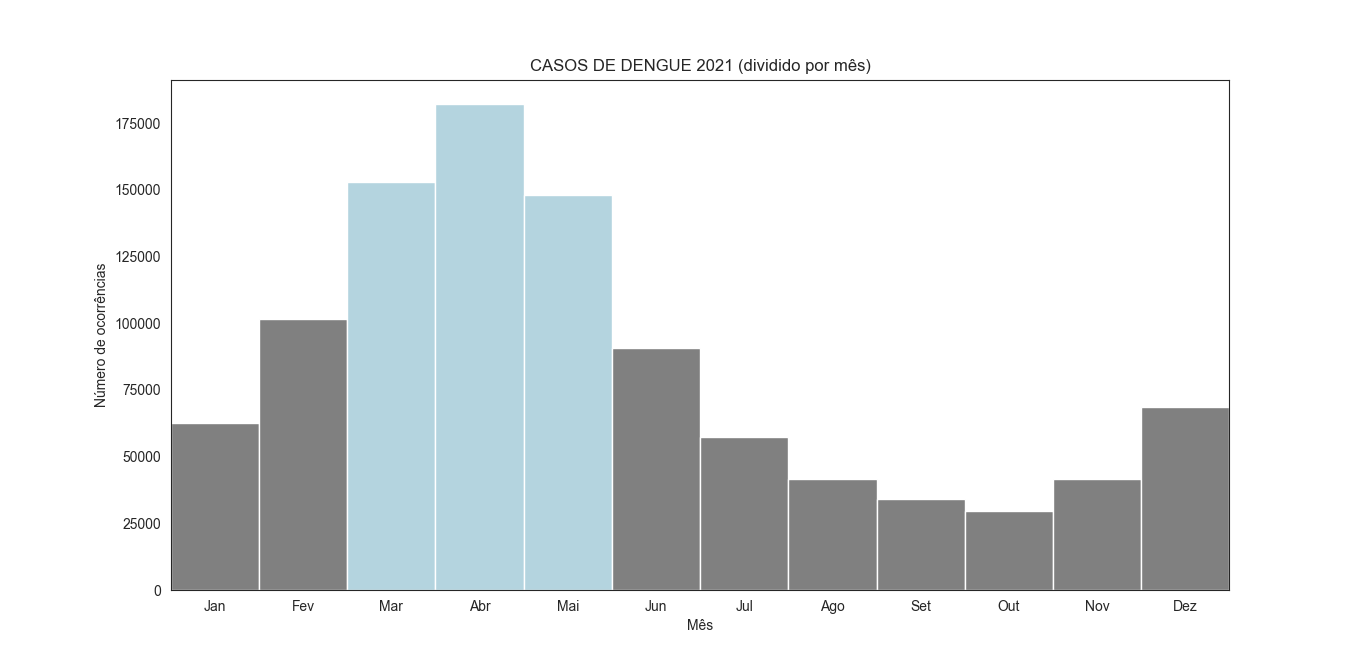
\includegraphics[width=\linewidth]{images/casos_dengue_2021.png}
        \caption{Casos de Dengue 2021}
        \label{fig:casos_2021}
    \end{minipage}
    \hfill % Espaço entre as imagens
    % Segunda imagem
    \begin{minipage}{0.45\textwidth}
        \centering
        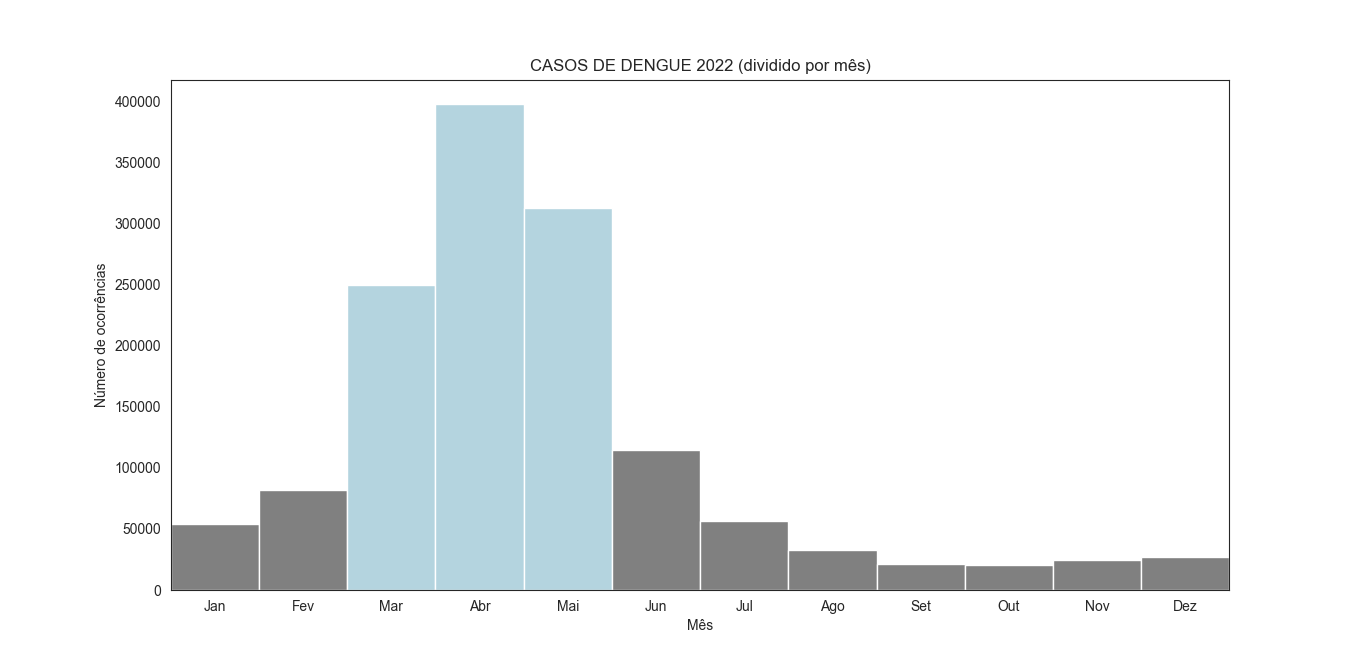
\includegraphics[width=\linewidth]{images/casos_dengue_2022.png}
        \caption{Casos de Dengue 2022}
        \label{fig:casos_2022}
    \end{minipage}
\end{figure}

\begin{figure}[h]
    \centering
    % Primeira imagem
    \begin{minipage}{0.45\textwidth}
        \centering
        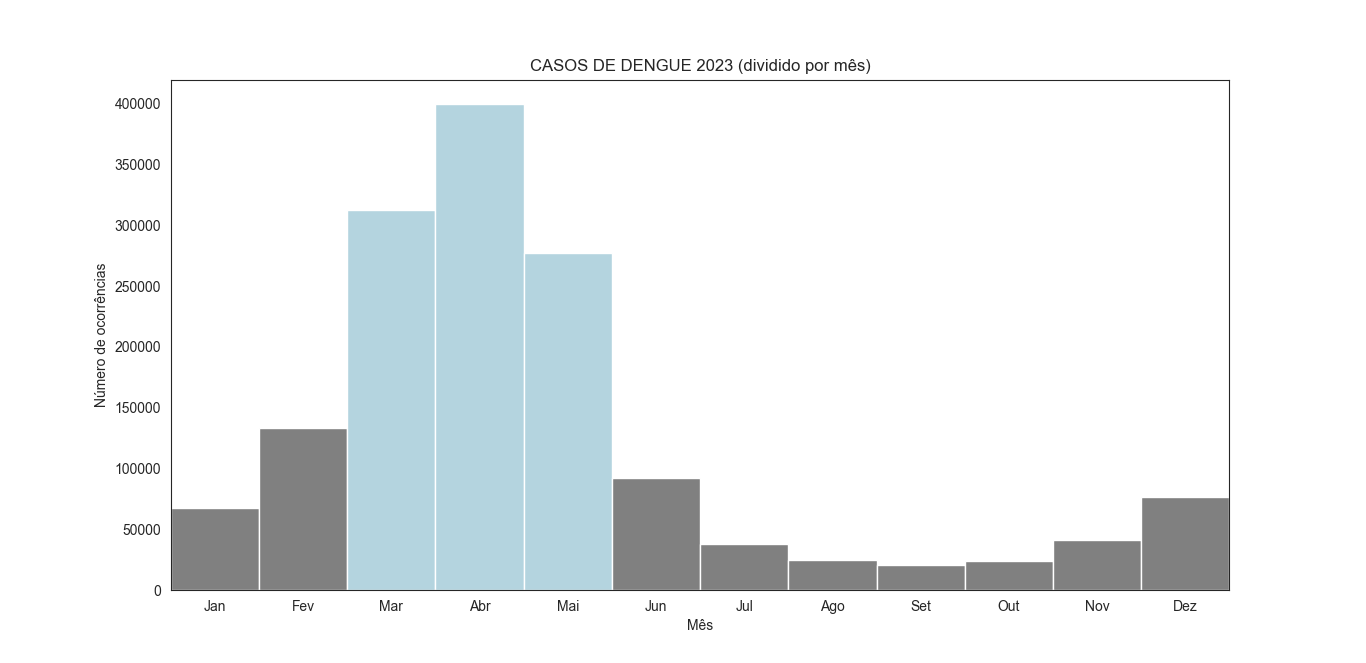
\includegraphics[width=\linewidth]{images/casos_dengue_2023.png}
        \caption{Casos de Dengue 2023}
        \label{fig:casos_2023}
    \end{minipage}
    \hfill % Espaço entre as imagens
    % Segunda imagem
    \begin{minipage}{0.45\textwidth}
        \centering
        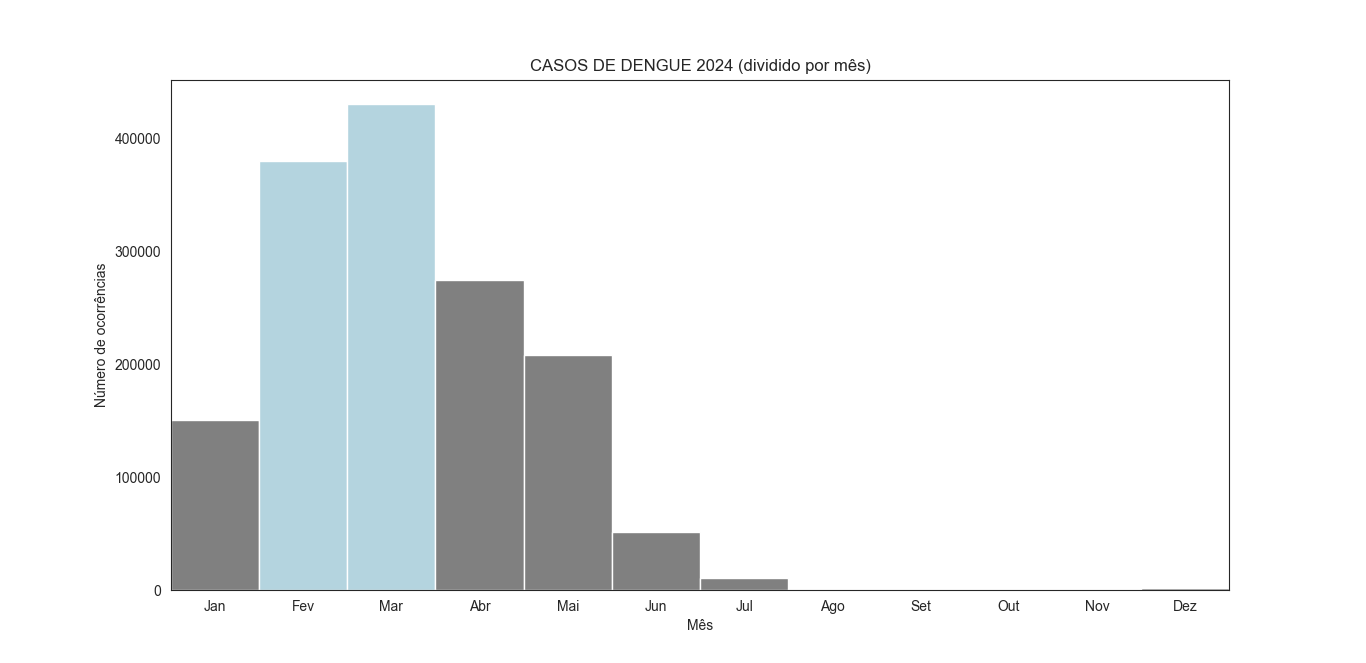
\includegraphics[width=\linewidth]{images/casos_dengue_2024.png}
        \caption{Casos de Dengue 2024}
        \label{fig:casos_2024}
    \end{minipage}
\end{figure}

\begin{figure}[H]
    \centering
    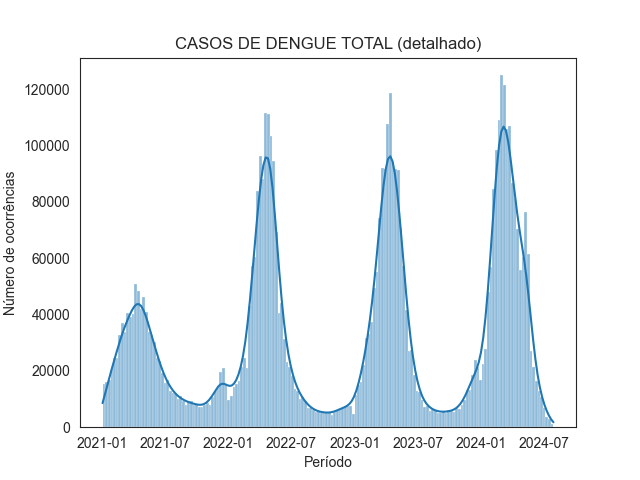
\includegraphics[width=0.95\linewidth]{images/casos_dengue_total.png}
    \caption{Casos de Dengue total}
    \label{fig:casos_total}
\end{figure}

\usepackage
Portanto, podemos observar que existe um padrão temporal na ocorrência dos casos de dengue, em que os meses de março, abril e maio têm o maior pico das observações.

Além disso, continuando o desenvolvimento da hipótese, fizemos uma contagem dos casos totais e dos óbitos por Unidade Federativa (calculando também a taxa de mortalidade, realizando o quociente entre o total de óbitos e o total de casos). As observações podem ser analisadas nas figuras \ref{fig:total_uf} e \ref{fig:mortalidade_uf}.

\begin{figure}[h]
    \centering
    \begin{minipage}{0.48\textwidth} % Aumente para 0.45
        \centering
        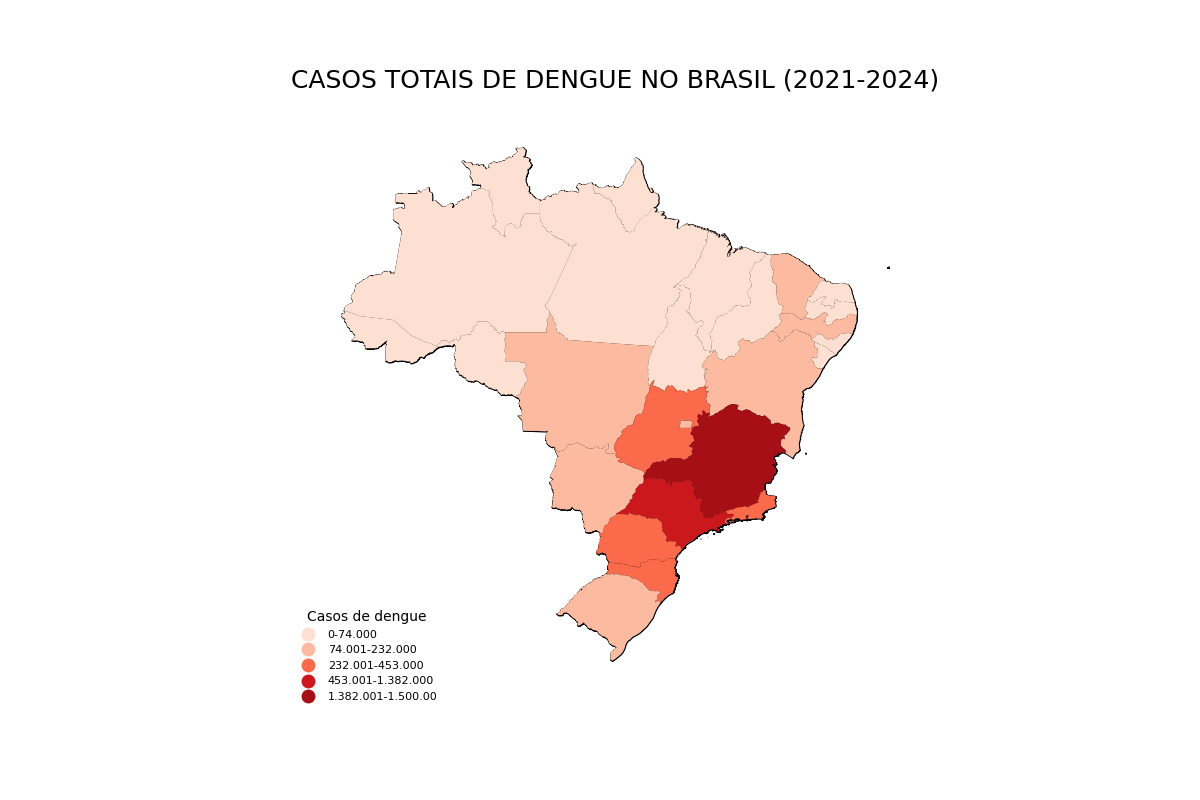
\includegraphics[width=\linewidth]{images/geoplot_total.png}
        \caption{Casos totais por Unidade Federativa}
        \label{fig:total_uf}
    \end{minipage}
    \hfill % Garante espaço entre as imagens
    \begin{minipage}{0.48\textwidth} % Aumente para 0.45
        \centering
        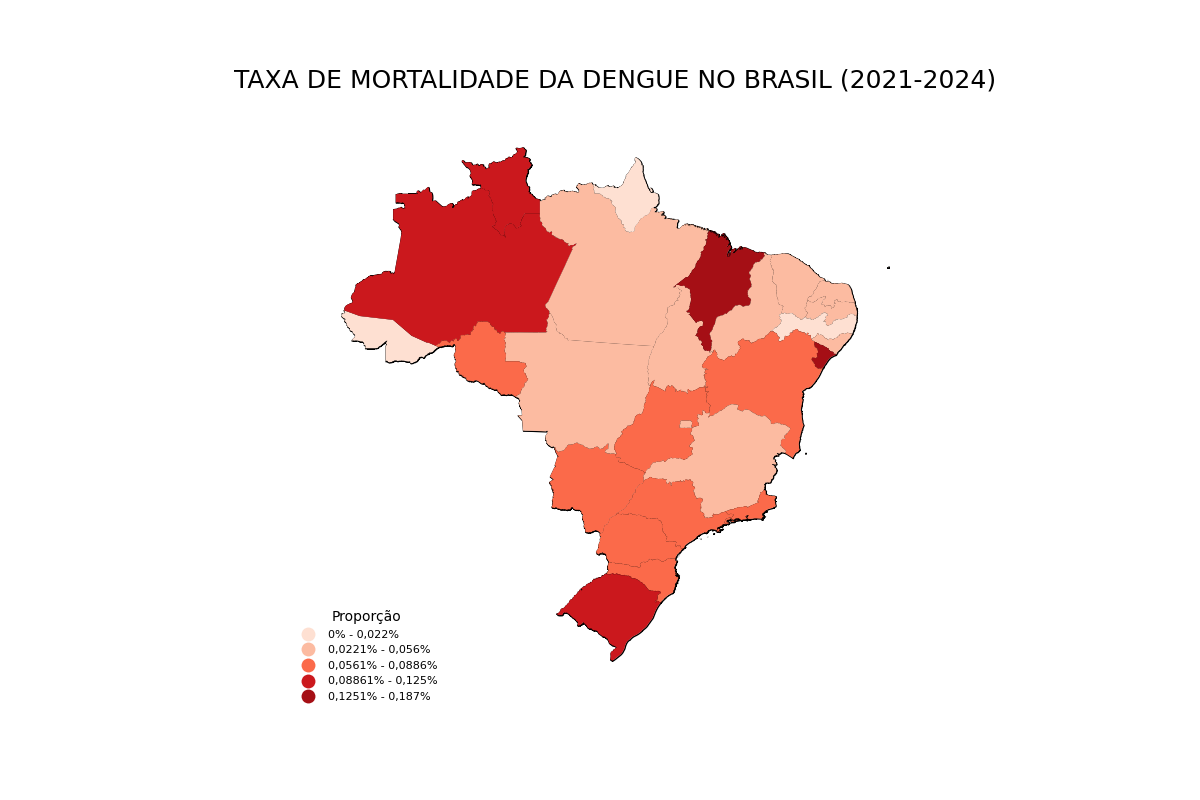
\includegraphics[width=\linewidth]{images/geoplot_mortalidade.png}
        \caption{Taxa de Mortalidade por Unidade Federativa}
        \label{fig:mortalidade_uf}
    \end{minipage}
\end{figure}

Logo, podemos presumir que, de acordo com a base de dados limitada utilizada, a Região Sudeste (destaque para Minas Gerais e São Paulo) apresentou o maior número de casos de dengue. Contudo, observando a taxa de mortalidade, os estados Amazonas, Roraima, Maranhão, Sergipe e Rio Grande do Sul obtiveram a maior concentração de óbitos por casos registrados de dengue. Para uma conclusão mais precisa, careceríamos de uma base com uma maior veracidade e abrangência do conjunto de dados.

\subsection{Hipótese 3}

\emph{"Sintomas mais graves se manifestam em um público mais velho?"}

Entender como os sintomas graves e leves afetam os pacientes de acordo com sua idade é de suma importância para tomada de decisões. Para realizar esta associação, primeiro foi feita uma separação dos sintomas registrados no dataset em classificações de acordo com sua periculosidade:
\vspace{0.5cm}
\\
\textbf{Sintomas Graves}: Sintomas que, quando manifestados, já representam um quadro clínico delicado do paciente
\begin{itemize}[nosep]
    \item[-] Renais: Prejudicação do sistema renal do paciente;
    \item[-] Hipertensão: Níveis de pressão arterial elevados;
    \item[-] Hepatopatia: Alteração do funcionamento natural do fígado;
    \item[-] Leucopenia: Diminuição no número de leucócitos (Glóbulos Brancos).
\end{itemize}
\vspace{0.5cm}
\textbf{Sintomas Preocupantes}: Quando percebidos, podem não ser um alerta imediato, mas podem evoluir para um quadro clínico mais grave
\begin{itemize}[nosep]
    \item[-] Vomito: Se é um sintoma muito recorrente, o paciente pode sofrer de desitratações severas;
    \item[-] Dor retroesternal: Sintoma incomum na dengue, pode representar um quadro mais grave da doença ou outras complicações não relacionadas à enfermidade;
    \item[-] Artrite: Dores, inflamações e prejuízo funcional nas articulações podem indicar quadros avançados da doença, o que pode requerir atenção maior para o paciente.
\end{itemize}
\vspace{0.5cm}
\textbf{Sintomas Comuns}: Normalmente, não representam uma futura ameaça, apenas em casos isolados
\begin{itemize}[nosep]
    \item[-] Febre: Reação defensiva comum do corpo a doenças;
    \item[-] Petequia: Pequenas manchas ou pontos vermelhos na pele, geralmente não representam um quadro grave da doença;
    \item[-] Mialgia: Dores musculares, são bem comuns em pacientes com dengue e não costumam representar uma ameaça futura;
    \item[-] Cefaleia: Dores de cabeça, sintoma comum da dengue;
    \item[-] Conjuntivite: Inflamação na conjuntiva, não representa uma ameaça grave ao estado de saúde do paciente;
    \item[-] Enxantema: Erupções cultâneas, sintoma corriquieiro em casos de dengue e não costuma representar estado alarmante do paciente;
    \item[-] Artralgia: Dores nas articulações corporais, tendem a não deixar sequelas após a recuperação do paciente;
    \item[-] Náusea: Tonturas e incômodo na parte superior do abômen, acompanhado de falta de apetite, relacionado a dengue, não representa uma enfermidade maior.
\end{itemize}

Após obter a classificação de cada sintoma, cada paciente teve um rótulo associado, este variando de acordo com a gravidade dos sintomas registrados:
\vspace{0.5cm}
\\
\textbf{CLASSIFICAÇÃO DOS SINTOMAS}
\begin{itemize}[nosep]
    \item[-] \textbf{Grave:} Se houve qualquer registro de um sintoma classificado como \emph{grave};
    \item[-] \textbf{Preocupante:} Se o paciente não teve nenhum sintoma grave, mas foi registrado um sintoma classificado com \emph{preocupante};
    \item[-] \textbf{Comum:} Caso o enfermo não tenha tido nenhum dos sintomas graves ou preocupantes, ou nenhum sintoma foi registrado
\end{itemize}
\vspace{0.5cm}
\hspace{1cm}Feita a separação dos pacientes de acordo com a gravidade dos sintomas, foi feita a plotagem de um boxplot que relaciona a idade dos pacientes dentro de cada categoria de classificação.

\begin{figure}[H]
    \centering
    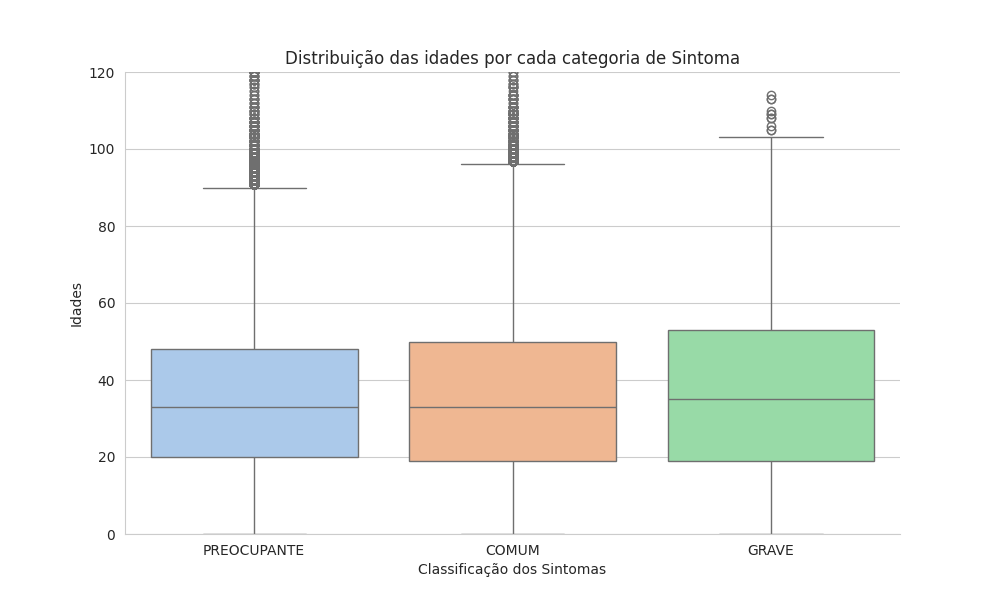
\includegraphics[width=1.0\textwidth]{images/ages_per_symptom_classification.png}
    \caption{Distribuição das idades por cada categoria de sintoma}
    \label{fig:occupation}
\end{figure}

Vale ressaltar que os enfermos com registros de sintomas preocupantes ou graves, mesmo que houvesse evidência da ocorrência de sintomas leves, ainda receberam a classificação dos riscos mais periculosos. Essa regulação foi feita tendo em vista que os sintomas mais graves são acompanhados dos sintomas leves, o que poderia ocasionar numa imprecisão na hora de calcular a relação entre as variáveis.

Analisando esse gráfico, conseguimos presumir, pela proximidade na distribuição de todas as categorias, que a gravidade do sintoma não tende a ser influenciada pela idade do paciente. Mas, para ter uma certeza, foi calculado o coeficiente R² para medir a correlação entre as duas variáveis.

Após o deferimento dos cálculos, foi obtido o valor de \(\approx 0.03\%\)

Esta porcentagem é um indicativo de \textbf{baixa relação} entre as variáveis, o que leva a conclusão de que, baseando-se nos dados disponíveis no dataset, e sabendo que o conjunto de dados é limitado e não abrange todos os casos e situações possíveis, os sintomas mais graves \textbf{possivelmente não} são influenciados diretamente pela idade do paciente. 

\subsection{Hipótese 4}

\emph{"Pessoas em ocupações relacionadas a zona rural têm maiores chances de contrair a doença?"}

Para essa análise, tendo em vista a existência de uma coluna que registra a ocupação de cada paciente no dataframe principal, foram utilizados os indícios sobre o trabalho que cada indivíduo realizava e sua possível contração de dengue. 

É sensato admitir que pessoas que trabalham no meio rural possuem maior chance de contraírem a dengue, pois suas ocupações estão mais predispostas a exposição ao ar livre, maior presença de criadouros e consequentemente água parada, menos infraestrutura e saneamento, além de menos controle sobre os vetores de propagação da doença.

Com essas informações, pode-se analisar a frequência que ocupações relacionadas ao meio rural aparecem no dataset e compará-las com outras ocupações gerais. Com este fim, foi feito um estudo seguindo estes passos: 
-  Obteve-se um dataset secundário retirado do site da CBO, Classificação Brasileira de Ocupações, que consta a relação do código contido no dataset principal e a descrição do seu título relacionando códigos em comum, auxiliando assim a associação por ocupações que continham termos relacionados ao meio rural, como "agro", "pecuária" e "rural".

Para uma análise mais fidedigna, foram removidos cargos com alcunhas "gerente", "economista", "diretor" e outros, pois, em hipótese, essas funções não possuem as mesmas predisposições comuns de outras profissões e portanto não devem entrar nas observações. Segmentando em dois conjuntos de dados, ocupações gerais e outros, realizamos cálculos para chegar na média de proporções de cada tipo de ocupação. Considerando a amostra que varia de 01/2021 até 07/2024, chegamos que a proporção das ocupações rurais é de aproximadamente 5 vezes maior que uma ocupação comum. 

Após as análises feitas acima, e, relembrando que as colunas do conjunto de dados utilizados no dataset não especifica exatamente o tipo de ocupação, e que foram feitas uma higienização dos dados para a realização da hipótese, evidencia-se um possível indício de que o trabalho de cada indivíduo influencia na sua chance de contrair a dengue, destacando-se a profissão de zona rural, tal qual mostrado no gráfico abaixo.

\begin{figure}[H]
    \centering
    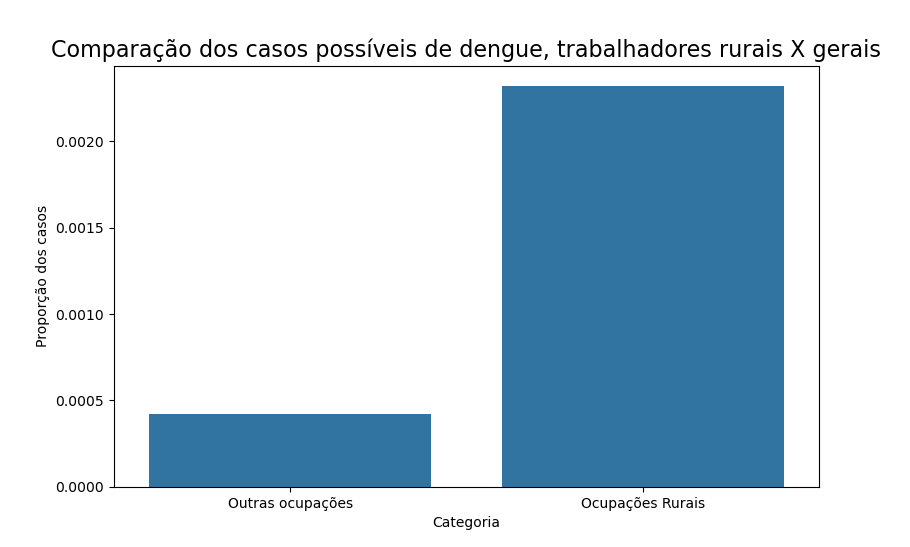
\includegraphics[width=0.6\textwidth]{images/plot_hp4.png}
    \caption{Distribuição das idades por cada categoria de sintoma}
    \label{fig:occupation}
\end{figure}


\subsection{Hipótese 5}

\emph{"Nos períodos de covid, houve alguma mudança em relação à quantidade de pessoas diagnosticadas com dengue? Além disso, nesses períodos, o tempo de demora entre a entrada no hospital e a hora do exame aumentou?
"}

Baseando-se no dataset no período coincidente com a pandemia de COVID-19, foram realizadas análises estatísticas básicas, incluindo o cálculo de quartis, desvio-padrão, média, entre outros, com o objetivo de comparar esses dados com o período pós-pandêmico. O propósito central dessas análises foi verificar a existência de uma possível relação entre o período pandêmico e um atraso no encerramento de casos de dengue, o que poderia sugerir que a pandemia do COVID-19 influenciou negativamente o controle e a gestão de outras doenças, como a dengue.

Com esse propósito, foi calculada a tabela que relaciona ambos os períodos em questão:


\begin{table}[H]
\centering
\caption{Comparação da diferença de dias entre a notificação da ocorrência até o encerramento do caso entre períodos }

\begin{tabular}{@{}l S[table-format=4.2] S[table-format=4.2]@{}}
\toprule
\textbf{Métrica}          & \textbf{01/01/21 - 30/11/22} & \textbf{30/11/22 - 31/07/24} \\ \midrule
Desvio Padrão                                 & 31.94              & 34.45              \\
Mediana (dias)            & 27.00              & 22.00              \\
1º Quartil (q1)           & 8.00               & 8.00               \\
3º Quartil (q3)           & 61.00              & 53.00              \\
Valor Mínimo (dias)       & 0.00               & 0.00               \\
Valor Máximo (dias)       & 505.00             & 545.00             \\
Total de Registros        & 2,987,188          & 2,356,590          \\
Soma dos Dias             & 102,288,377        & 75,412,113         \\
Média de Dias             & 34.24              & 32.00              \\ \bottomrule
\end{tabular}
\label{tab:comparison}
\end{table} \\

Após a análise das métricas calculadas, supõe-se que, de acordo com as datas disponíveis, não existe correlação entre os períodos pandêmicos pós-pandêmicos, pois a mensuração entre os dois períodos não resultou numa variação significante de resultado, tome como exemplo os quartis, que apresentam uma diferença baixa, quando o apresentam.

Por outro lado, poderíamos supor uma relação entre o aumento do intervalo de tempo entre a notificação dos casos e a realização dos exames, o que poderia indicar uma correlação entre a pandemia de COVID-19 e o atraso na condução de exames de outras doenças. 

De forma análoga a anterior, foi realizado o cálculo das principais métricas dos períodos em pauta:

\begin{table}[H]
\centering
\caption{Comparação da diferença de dias entre a notificação da ocorrência até a realização do exame de dengue entre períodos}
\begin{tabular}{@{}l S[table-format=3.2] S[table-format=3.2]@{}}
\toprule
\textbf{Métrica}          & \textbf{01/01/21 - 30/11/22} & \textbf{30/11/22 - 31/07/24} \\ \midrule
Desvio Padrão  & 31.64              & 28.46              \\
Mediana (dias)            & 12.00              & 12.00              \\
1º Quartil (q1)           & 4.00               & 4.00               \\
3º Quartil (q3)           & 30.00              & 37.00              \\
Valor Mínimo (dias)       & 0.00               & 0.00               \\
Valor Máximo (dias)       & 545.00             & 465.00             \\
Total de Registros        & 646,233            & 886,315            \\
Soma dos Dias             & 14,496,361         & 20,920,025         \\
Média de Dias             & 22.43              & 23.60              \\ \bottomrule
\end{tabular}
\label{tab:comparison}
\end{table} 

A seguir da aferição dos dados, constata-se que, pelas mesmas condições da limitações dos dados anterior, as diferenças das medidas calculadas não significam uma correlação válida o suficiente, visto que as diferenças são mínimas. Note, por exemplo, a pequena diferença entre o desvio padrão e a média, bem como outras estatísticas que se mostram equivalentes. 

\section{Conclusão}


Este estudo explorou a relação entre os casos de dengue no Brasil, seus impactos, sintomas e os fatores externos, como a pandemia de COVID-19 e as condições ocupacionais, no período de 2021 a 2024. A partir da análise de dados disponibilizados pelo SINAN, foi possível identificar padrões epidemiológicos e validar ou refutar hipóteses iniciais.
Por fim, embora este estudo tenha gerado contribuições relevantes, é crucial reconhecer suas limitações. Entre elas estão a falta de especificidade em algumas colunas do dataset, a presença de colunas com dados ausentes, a compreensão insuficiente sobre o contexto de coleta dos dados escolhidos e outros déficits detalhados em cada hipótese analisada. Espera-se que estudos futuros possam investigar novos conjuntos de dados ou ampliar as análises, incorporando variáveis adicionais para promover uma compreensão mais profunda dos impactos dos casos de dengue no Brasil.


\printbibliography[title={Referências}]

\end{document}
